\section{Quantisierung endlicher Wortl�ngen}
Das Quantisierungsrauschen ist ein nichtlinearer deterministischer Prozess. Dies ist mit den g�ngigen mit den g�ngigen Mitteln kaum zu rechnen, deshalb wird das Quantisierungsrauschen durch eine lineare stochastische Rauschquelle ersetzt.
\begin{minipage}{6.5cm}
\begin{tabular}{c}
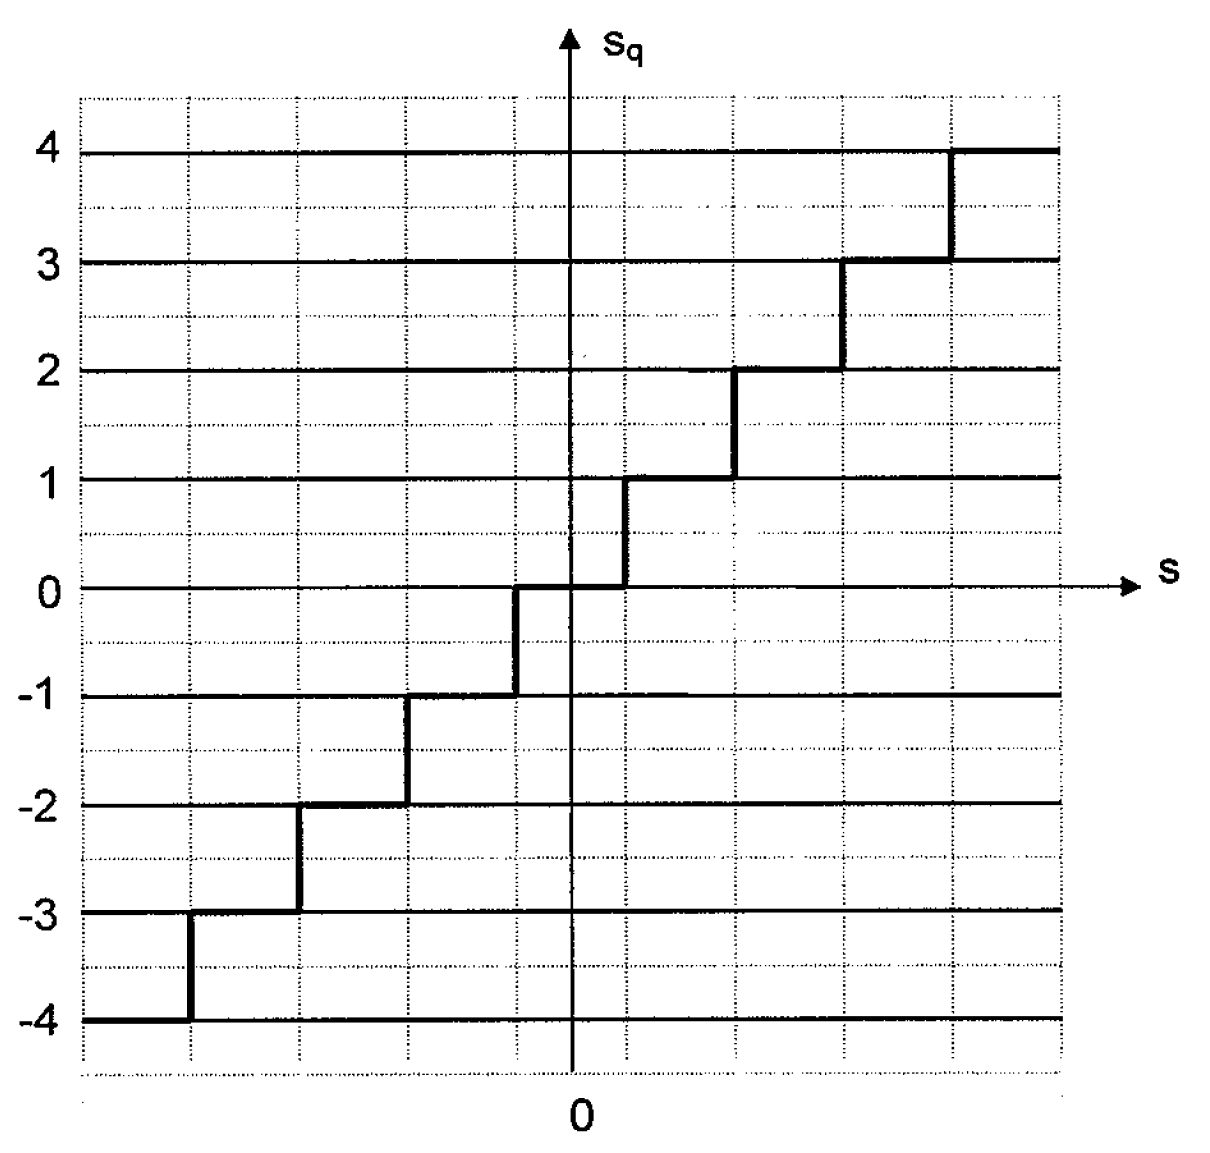
\includegraphics[width=6cm]{Content/QuantRausch/Quantisierung.png}\\
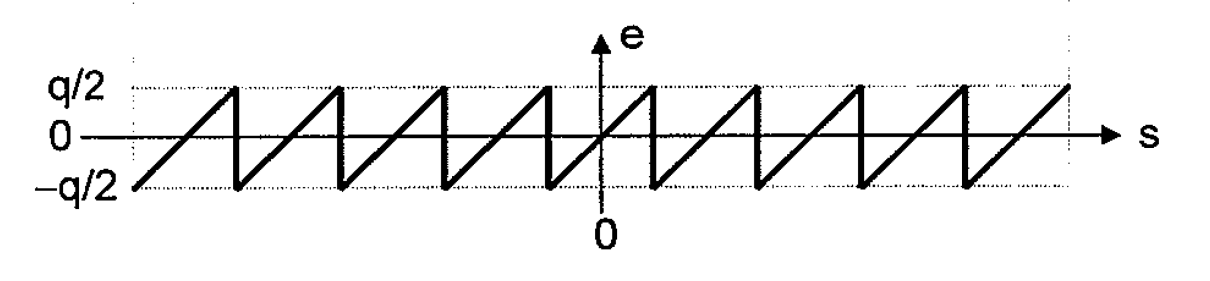
\includegraphics[width=6cm,trim= 1cm 0cm 0cm 0cm]{Content/QuantRausch/Quantisierungsrauschen.png}
\end{tabular}
\end{minipage}
\begin{minipage}{12cm}
	\begin{minipage}{5.5cm}
	\textbf{nichtlinear deterministisch:}\\
	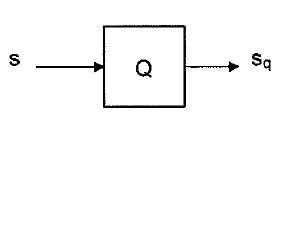
\includegraphics[width=4cm,trim=0cm 3cm 0cm 0cm]{Content/QuantRausch/Quant.png}\\
	\textbf{linear stochastisch:}\\
	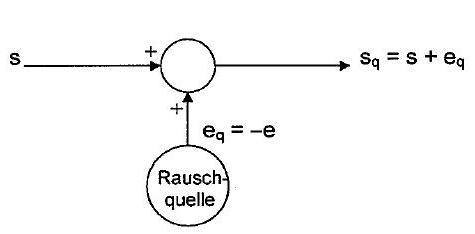
\includegraphics[width=5cm]{Content/QuantRausch/RauschLin.png}\\
	\end{minipage}
	\begin{minipage}{6.5cm}
	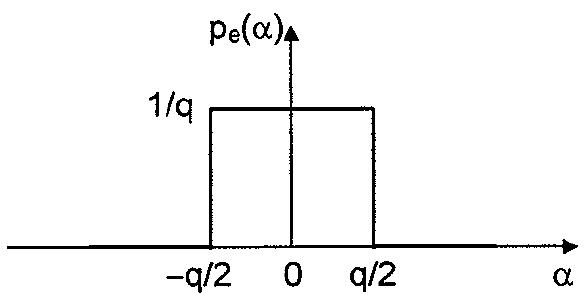
\includegraphics[width=5.0cm,trim= 0cm 1cm 0cm 0cm]{Content/QuantRausch/Quantisieren02.JPG}\\
	\center
	$\mu_m=\int\limits_{-\infty}^{\infty}{\alpha^m\cdot p_e(\alpha)d\alpha}$\\

	$\mu_1=0$\\
	$P_e=\sigma_e^2=\mu_2=\frac 1q \int\limits_{-q/2}^{q/2}{\alpha^2\cdot p_e(\alpha)d\alpha}$\\
	Gleichverteilt ($q<<\sigma$):
	$P_{eGV}=\frac{q^2}{12}$\\
	\end{minipage}
	
	\vspace{0.5cm}
	
	$SNR=10\cdot log(P_s/P_e)=K+20\cdot n \cdot log(2)= K+6.02\cdot n$\\
\end{minipage}

\begin{minipage}{8.5cm}		
	\begin{tabular}{| p{3.5cm} | p{2cm} | p{1.4cm} |}
					\hline
					Vert.dichtefkt. des Signals & $P_e$ & K \\
					\hline
					\hline
					Gleichverteilt & $A_{pp}^2/12$ & 0dB \\
					\hline
					Sinusf�rmig & $(A_{pp}/2)^2/2$ & +1.67dB  
					\\
					\hline
					Gauss'sche Vert. & mit $\sigma^2$ der �berst.$<10^{-5}$ & -8.5dB  
					\\
					\hline
	\end{tabular}
\end{minipage}
\begin{minipage}{7cm}
$q=A_{pp}/N = A_{pp}/2^B$

q: Quantisierungsstufenh�he\\
n: Wortl�nge (Bit/Abtastwert)\\
$A_{pp}$: Tot. Aussteuerungsbereich\\
$P_{s}$: Signalleistung\\
$P_{e}$: Quantisierungsrauschleistung\\
\end{minipage}

\subsection{Leistungsdichtespektrum des Quantisierungsfehlers}
%\scriptsize
$\rightarrow$Quantisierungsfehler ist zeitdiskretes, gleichverteiltes, weisses
Rauschen.\\

    \begin{minipage}{8cm}    	
			\textbf{Diskrete Autokorr.:}\\
			$R_{ee}(k)=\dfrac{q^2}{12}\delta(k)=\begin{cases}q^2/12 & k=0 \\0 &
			\text{sonst} \end{cases}$\\
			
			Spektrale Leistungsdichte:\\
			$N_{oe}/2 = P_e/f_0 = q^2/(12f_0)$\\
    \end{minipage}
    \begin{minipage}{11cm}    	
			\textbf{Kontinuierl. Autokorr.:}\\
			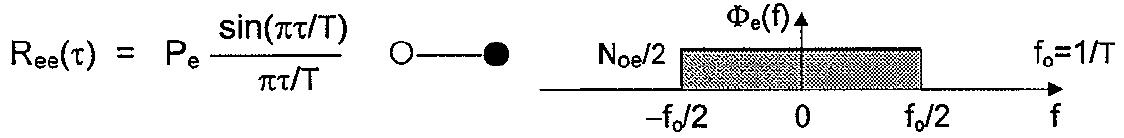
\includegraphics[width=11cm]{Content/QuantRausch/Quantisieren03.JPG}\\
			$\rightarrow$Fl�che des $\Phi_e(f)$-Rechtecks entspricht $P_e$\\ \\

    \end{minipage}\\
		
    \begin{minipage}{8cm}    	
			\textbf{AKF des Quant.-fehler:}\\
			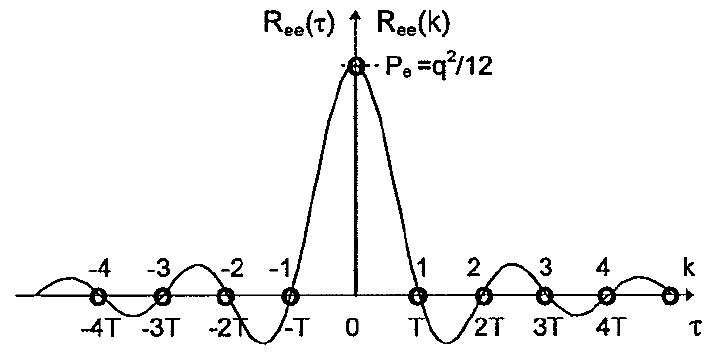
\includegraphics[width=8cm]{Content/QuantRausch/Quantisieren04.JPG}\\
    \end{minipage}
    \begin{minipage}{11cm}    	
			\textbf{Leistungsdichtespektrum des diskreten Quant.-fehlers:}\\
			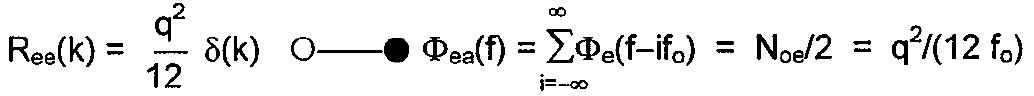
\includegraphics[width=11cm]{Content/QuantRausch/Quantisieren05.JPG}\\
			$\rightarrow f_0$ = spektrale Periode\\
			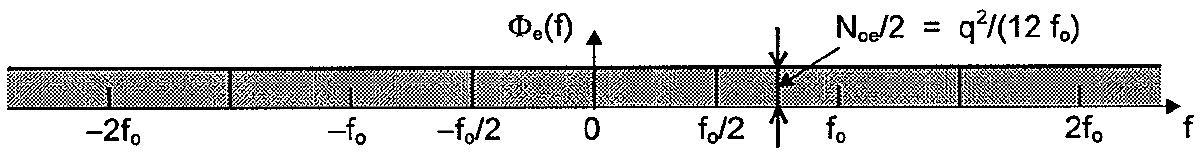
\includegraphics[width=11cm]{Content/QuantRausch/Quantisieren06.JPG}
			
			\vspace{1.2cm}
			
    \end{minipage}
	\normalsize



\vspace{-1cm}
\subsection{Quantisierung der Filterkoeffizienten}
    \begin{minipage}{13.5cm}    	

		
		\begin{liste}
	 		\item Durch Begrenzung der Wortl�nge sind Lage der Pole/Nullst. gering
			abweichend. Pole ev. ausserh. Einheitskr.
	 		\item Keine Nichtlinearit�ten wie bei Signalquant.
	 		\item Ver�nderung der �bertr.-Fkt. durch Quantisierung ist von der
	 		Filterstrukt. abh�ngig
		\end{liste}
		Allgemein:\textbf{Wenig empfindlich sind Strukt., bei denen 
		wenige Koeff. die Lage weniger Pole und Nullst. beeinflussen.}\\
    \end{minipage}
    \begin{minipage}{4.5cm}    	
			\scriptsize 
			%\footnotesize
			\begin{tabular}{| p{2.8cm} | p{1.5cm} | }
            	\hline
            	Filterstruktur & Beurteilung  \\
            	\hline
            	\hline
            	Direkte Form I und II & schlecht  \\
            	\hline
            	Parallelstruktur & schlecht
            	\\
            	\hline
            	Kaskadenstruktur & gut
            	\\
            	\hline
            	Reines FIR-Filter & schlecht 
            	\\
            	\hline
            	Kreuzgliedfilter & gut
            	\\
            	\hline
			
	\end{tabular}
	\normalsize
\end{minipage}
